\documentclass[withoutpreface]{cumcmthesis}
\title{基于logisim的多周期MIPSCPU硬布线控制器设计}
\usepackage{graphicx} 
\begin{document}
\maketitle
\begin{tabular}{cccccc}
	\hline
	学  号 & E12214052 &专  业 & 计算机科学与技术 &姓  名 & 赵宸宇 \\
	\hline
	实验日期 & 2024年9月26日 &教师签字 &  &成  绩&\\
	\hline
\end{tabular}
\begin{abstract}
	基于前两次实验报告中提出的\textbf{工作展望},在本次附加实验对其进行\textbf{实现}。
		
	在前一次实验中,我完成了纯硬控制器的设计工作。但没有处理历史遗留的数据通路不美观的问题。这个问题将在本次实验中得到解决。
	
	本次实验\textbf{在第二次实验}“多周期微程序mips处理器设计”\textbf{已经完成}数据通路设计和\textbf{“纯”硬布线控制器设计的基础上},着重对\textbf{数据通路}和\textbf{微命令字段}进行了\textbf{重构}。目的是增加电路的鲁棒性、修复历史小错误、增加电路美观程度。经过本次附加实验的重构工作,学生对CPU工作原理理解更加深刻,设计的电路更美观,更耐用了。

\subsection*{本次实验的实验产出有:}
\begin{enumerate}
	\item 数据通路(2张)完全重构的电路图;见实验2.2文件夹
	\item tex\textbf{附加实验的实验报告}
	\item \textbf{支撑材料}(用于命令字段重构的xlsx表格、py程序、分析记录等)
	\item \textbf{头哥}网再次通关(用于测试重构的电路)
	\item \textbf{gitee}仓库增量更新 请见\url{https://gitee.com/cslearnerer/AHU-CSHT}
\end{enumerate}
\end{abstract}
\tableofcontents
\newpage
\section{【实验目的】}
1. 对第一版\textbf{数据通路进行重构},以提升性能,\textbf{美化外观},\textbf{划分功能区};

2. 对第一版控制电路的\textbf{ALUOP硬件电路}和\textbf{微命令字段}中存在的和MOOC视频中不一样的地方,通过修改,和MOOC进行统一。(即我个人使用的ALUOP的\textbf{11控制信号对应了MOOC中的10控制信号},虽不造成电路运行错误,但是应当纠正)

3. 对\textbf{微命令字段进行简化},更改ALUOP的11信号为10信号;

4. \textbf{测试调通}新电路

\section{【实验内容】}
\subsection{数据通路重构}
	通过一下午的绘图、测试,数据通路的各项指标都得到了极大改善。
% TODO: \usepackage{graphicx} required
\begin{figure}[!h]
	\centering
	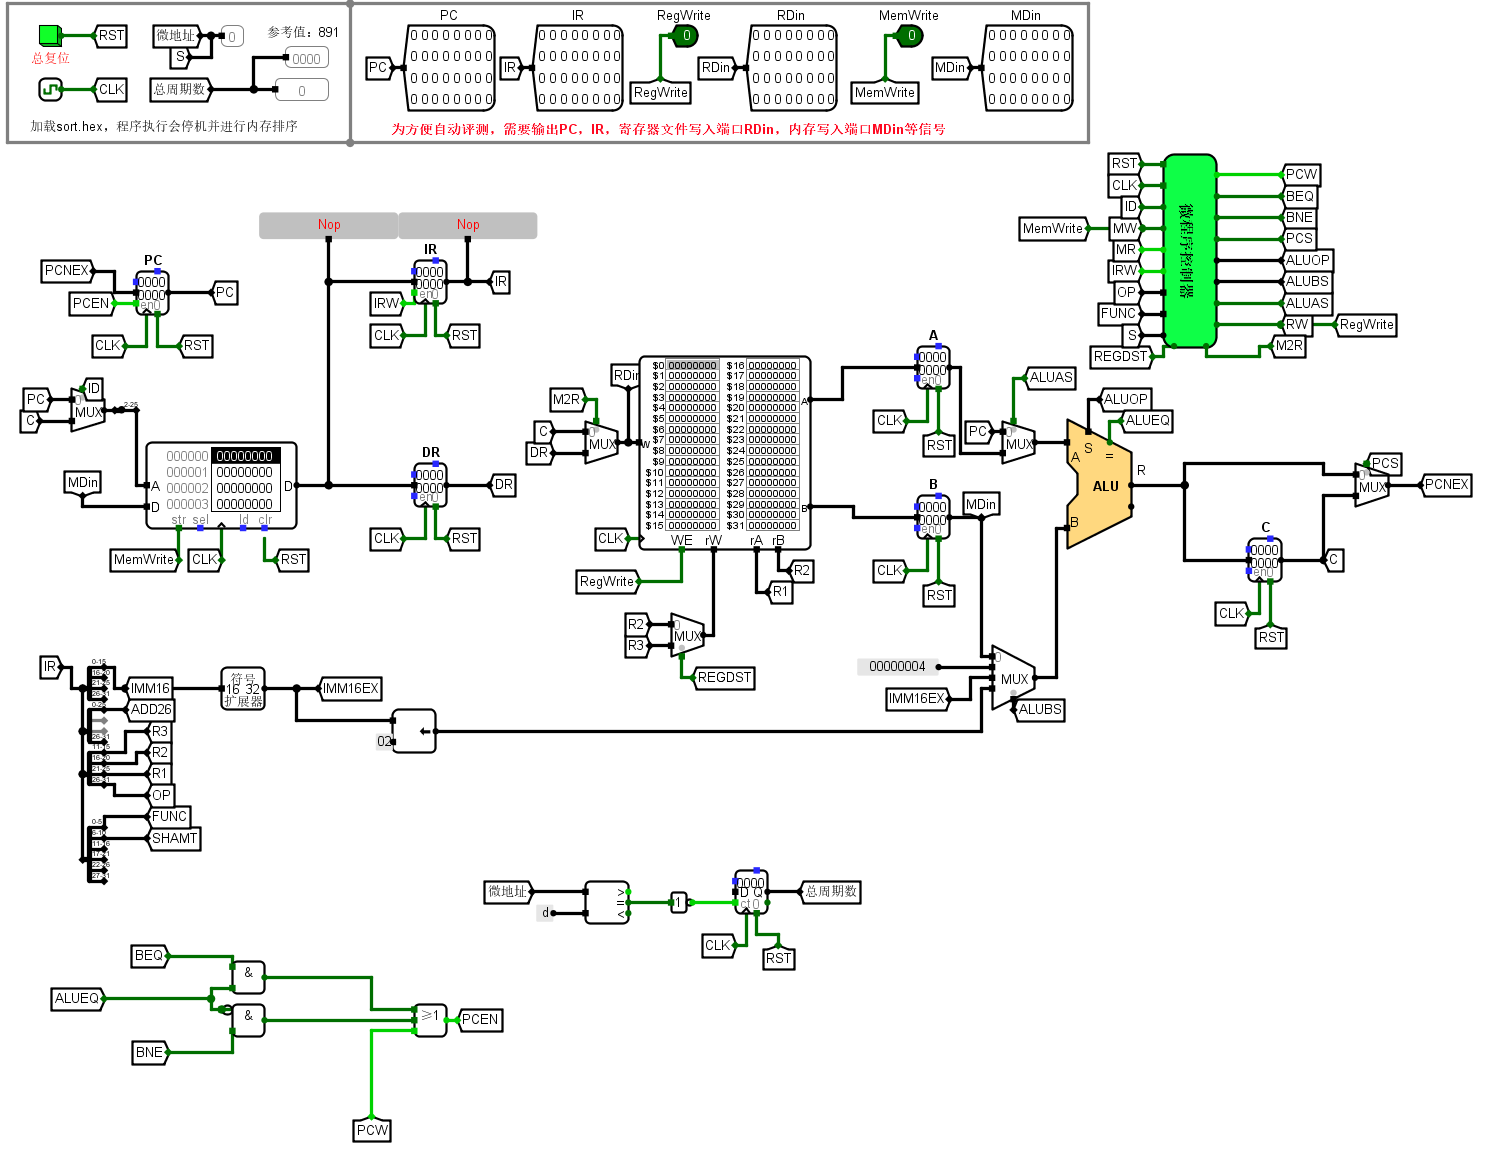
\includegraphics[width=0.7\linewidth]{新通路}
	\caption[数据通路重构]{}
	\label{fig:datar_re}
\end{figure}
	如\cref{fig:datar_re}所示,数据通路被划分为了存储区(左侧第二行)、地址区(左第一行)、指令拆析区和立即数解析区(左3)、地址载入布尔值计算区(左4)、reg堆(中央)、AB锁存器和ALU计算区(右侧中间)、控制逻辑区(右上)。
	
	通过将数据通路按功能进行划分,可以在之后的工作中很方便地对各个模块进行维护、增删改查。
\subsection{微命令字段重构}
	\begin{figure}[!h]
		\centering
		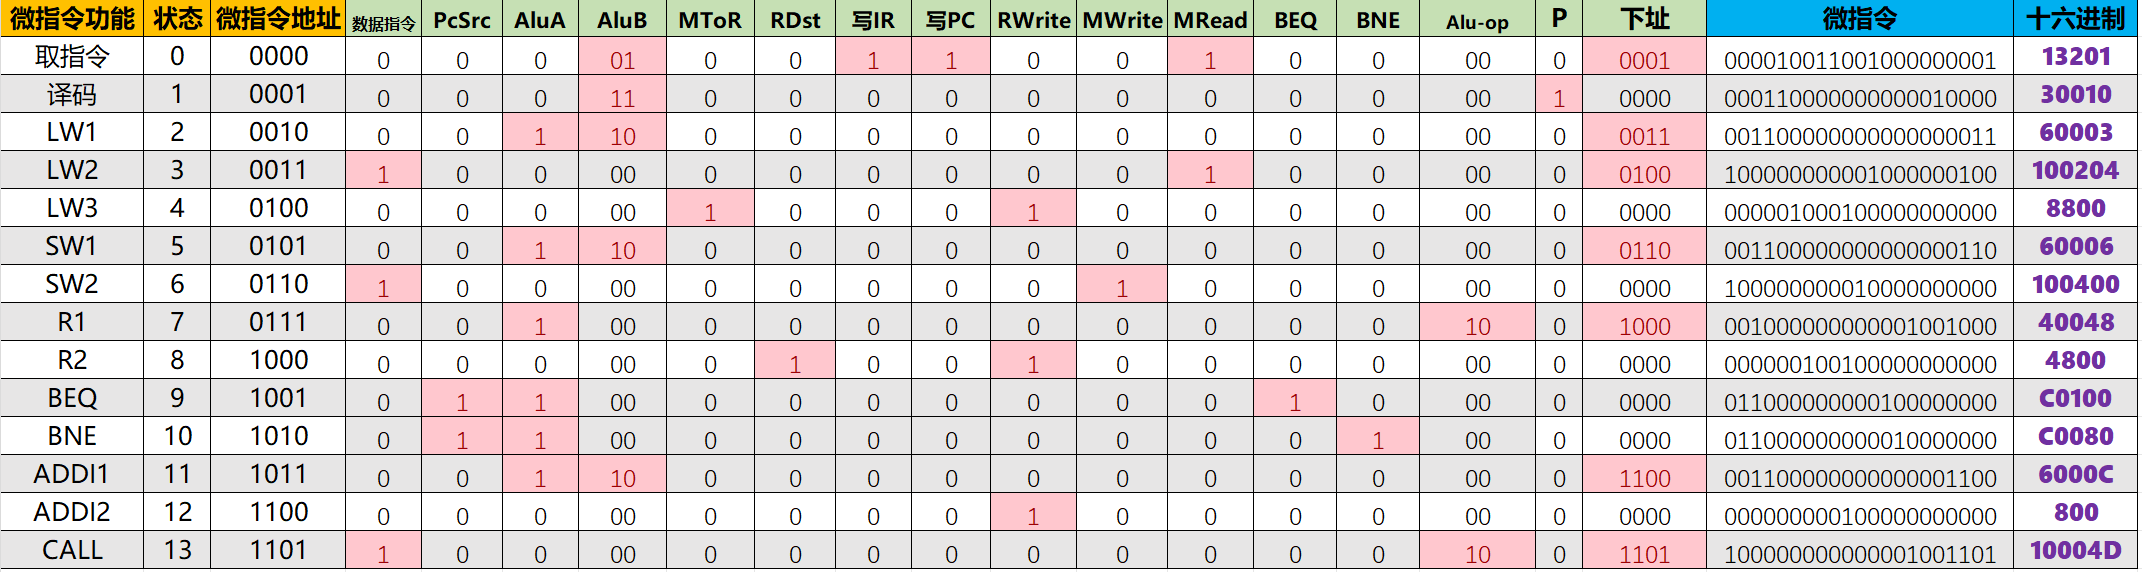
\includegraphics[width=0.7\linewidth]{新字段}
		\caption[微命令字段重构]{}
		\label{fig:microIseg_re}
		如\cref{fig:microIseg_re}所示,在新的字段中,ALUOP的值和MOOC规范相统一。从原先采用值00-加,01-减,11-由Func决定,变为了00-加,01-减,10-由Func决定。后面的方案和课程设计相统一,体现电路设计规范性。
	\end{figure}
\subsection{头哥网再次通关}
	在重构完数据通路、控制电路(alu部分)、微命令字段相关的微程序组件和硬布线组件后。
	
	我去头哥网做了重构后测试,得到以下结果:
	\begin{figure}[!h]
		\centering
		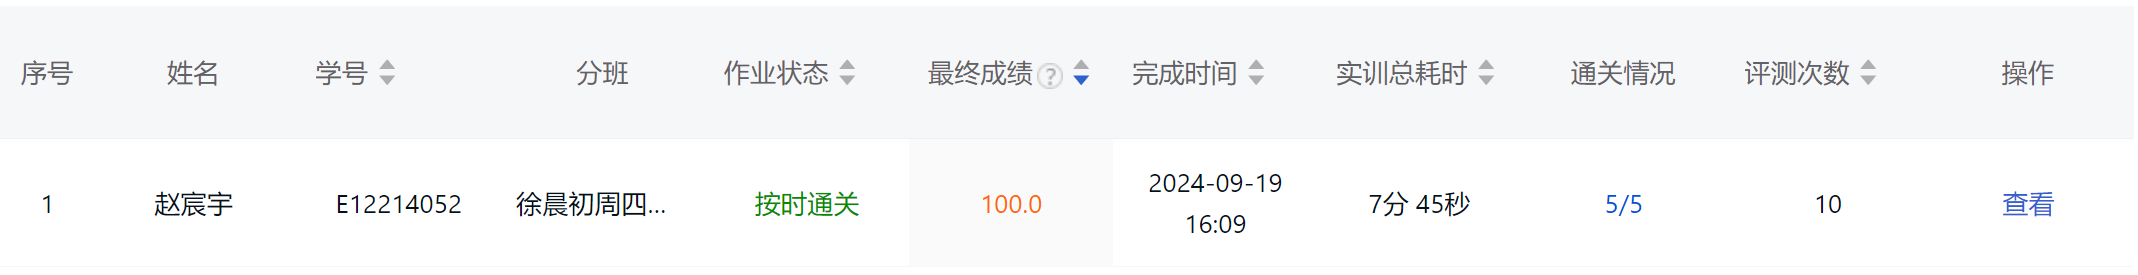
\includegraphics[width=0.7\linewidth]{重构测试通过}
		\caption[重构测试通过]{}
		\label{fig:pass}
		如\cref{fig:pass}所示,新的电路设计是完备的。
	\end{figure}
\subsection{gitee记录}
	最后,我将以上实验记录包括本报告放入实验2.2文件夹,并将记录push到gitee。
	
\section{【小结讨论】}
	通过本次实验,电路的鲁棒性、修复历史小错误、增加电路美观程度增加。学生对CPU工作原理理解更加深刻,设计的电路更美观,更耐用了。
\end{document}